\chapter{Graph Neural Networks}
\label{ch:gnns}

The philosophy behind graph neural networks (GNNs) is rooted in the idea that nature is best understood when broken down into compositional elements.
By understanding these elements and the rules governing their interactions, we can gain insights into the system as a whole.
This reductionist approach is used in many areas of science, and indeed is the basis for all of particle physics.

Graphs serve as a prime example of explicitly structured data, encompassing entities and their pairwise relationships. GNNs are a type of deep learning model designed to handle this structure, allowing information to flow through the network in a manner that mirrors the graph's organization.

This chapter explores the foundational principles of GNNs, how they operate, and their limitations.
It also delves into the most successful GNN variant to date, the transformer model, which is utilized extensively in the subsequent chapters of this thesis.
This chapter follows the notation and formalism of~\textcite{RelationalInductiveBiases}.

\section{Learning Relations}

Relational reasoning~\cite{SimpleNeuralNetwork} is the development of rules that describe how the properties of entities modify the relations between them, and how in turn the relations modify the properties of the entities.
GNNs employ relational reasoning to complete tasks by directly manipulating the rules, entities, and relations of a system.

An example of successful relational reasoning being used in deep learning outside GNNs is in image processing tasks.
An image is typically represented as a rank-3 tensor using the pixel values as the tensor elements.
This tensor of has shape $(H, W, C)$, where $H$ and $W$ describe the image resolution, and $C$ is the number color channels.
If one wanted to process this tensor with an MLP, it must first be flattened to a have of shape $H \times W \times C$.
Within each affine layer every element of the input tensor is connected to every element of the output tensor.
While this leads to a flexible model, it also destroys the spatial structure of the image and no reusable relationships or rules are used.

Alternatively, we could use a network composed of learnable convolutional kernels.
These kernels scan over the input tensor, computing the weighted sum of the elements within the kernel window.
This introduces two key relational inductive biases: locality and translation invariance.
Locality refers to the assumption that the relationship between two elements is stronger if they are close together in the input space.
Translation invariance refers to the assumption that the relationship between two elements is the same regardless of their absolute position in the input space.
Locality is enforced by using a kernel width of limited size and translation invariance is enforced by reusing the same kernel across the whole image.
Each convolutional kernel defines rule for how elements within the structure of the input tensor are related.

This is an example of geometric deep learning, also called a relational inductive bias, whereby the known structure of the data is embedded into the architecture of the model itself, rather than being learned directly from the data.
This reduces the number of parameters required in the model, allowing for more statistically efficient learning.

\section{Defining a Graph}

A graph $\mathcal{G}$ is a data structure that consists of a set of $N$ attributed nodes $\mathcal{N} = \{\x_i\}_{i=1}^{N}$ interconnected by a set of $N^e$ attributed edges $\mathcal{E} = \{(\x_k, r_k, s_k)\}_{k=1}^{N^e}$.
Here $\edge_k$ are the edge attributes, and $s_k$ and $r_k$ are the indices of the sender and receiver nodes in $\mathcal{N}$ respectively.
It is also useful in many contexts to define a global attribute $\u$ which describes the graph as a whole.
A singular-graph can be represented as a tuple $\mathcal{G} = (\mathcal{N}, \mathcal{E}, \u)$.
The structure of the graph is only defined by the interconnections between the nodes, the actual ordering of the nodes in the set is arbitrary.
Therefore, any operation on the graph should not depend on this order.
Note that the adjacency matrix of the graph is not explicitly defined, but can be inferred from the elements of $\mathcal{E}$.

This description of a graph is very general and each of the terms $\mathcal{N}$, $\mathcal{E}$, and $\u$ are optionally included.
We could allow multiple sets of edges to exist between nodes $\{\mathcal{E}^1, \mathcal{E}^2, \ldots\}$, defining a multi-graph.
Each of the edge $\x_i$, node $\edge_{k}$, and global $\u$ attributes can also be encoded as any type of representation, even graphs themselves.
In most use cases dealt with in this thesis, each of $\x_i$, $\edge_k$, and $\u$ are real valued tensors.
It is also common for all the nodes to share the same dimensionality, and the same for the edges, imposing an equivalence between the elements of the set.
This it simplifies the design of the model as it allows operations on the individual elements to be parameterized with standard building blocks, such as affine layers, MLPs, and CNNs.

Representing a graph in code requires tuple or dictionary of real valued tensors $(\x, \edge, \u)$.
Here, $\x \in \mathbb{R}^{N \times d}$, $\edge \in \mathbb{R}^{N \times N \times d_e}$, and $\u \in \mathbb{R}^{1 \times d_u}$, where $d$, $d_e$, and $d_u$ are the dimensionality of the node, edge, and global features respectively.
The edge matrix is typically ordered such that $\edge_{ij}$ is the edge from node $i$ to node $j$.
To represent the existence or absence of an edge between two nodes, a binary adjacency matrix $\mathbf{A} \in \{0, 1\}^{N \times N}$ can be used where $\sum{\mathbf{A}} = N^e$.
Alternatively, one could use a sparse tensor representation, which is more memory efficient but can complicate the implementation of the model.

Almost all GNNs operate by facilitating message passing between the nodes of the graph.
In this framework each node sends messages to their neighbours.
These messages are then aggregated and used to update the node's attributes.
Exact details of how this is done can vary between models, but the core idea is the same.

\begin{figure}
    \centering
    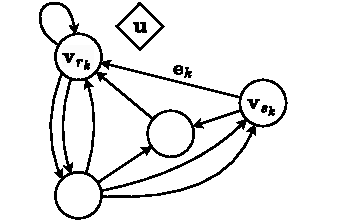
\includegraphics[width=0.5\textwidth]{Figures/graph_networks/graphs.pdf}
    \caption{A directed multi-graph with node, edges a global attribute $\u$. Highlighted is the edge $\edge_{k}$ which connects the sender node $s_k$ to the receiver node $r_k$.}
    \label{fig:graph}
\end{figure}

\section{Graph Type Data}
\label{sec:graph_data}

Graph or set representation is fairly ubiquitous in the real world as it may be used for anything that can be broken down into discrete elements.
For instance, a collection of particles captured by a detector can be expressed as sets, where the stable particles are the nodes and their attributes are the particle kinematics.
This is a natural representation because, for a single collision event, there is no inherent ordering to the outgoing particles.
This is natural representation as for a single collision event, there is no inherent ordering to the outgoing particles.
Some other examples are shown in \Cref{fig:graph_examples}.
Particle interactions and decay chains, such as the all-hadronic $ttH$ production process shown in \Cref{fig:feynman}, can be represented as a graph.
In this situation, it might be more natural to represent the particles in the Feynman diagram as edges rather than the nodes.
Chemical compounds can also be easily represented as graphs, where the atoms are the nodes and the chemical bonds between them are the edges.

Even data which is not inherently graph-like can be broken down into constituent parts and interconnected to form a graph.
Text can be \textit{tokenized} by treating words or subwords as nodes~\cite{Attention} and images may be segmented into patches \Cref{fig:dog}.
Though graphs typically have no natural ordering, text and image patches would not make sense if shuffled, thus order has to be imposed by the model.
This can be done by including the position of the node in its attributes or limiting the edges to only connect the nodes in a predetermined order.
This is covered in more detail in \Cref{sec:edge_biases_sequences}.

In analysing graph data within real-world contexts, there exists three primary types of predictive tasks: graph-level, node-level, and edge-level predictions.
For graph-level tasks, the aim is to predict an attribute or property that encompasses the entire system as a whole.
An example of this in the context of computer vision would be the classification of the entire image.
Node-level tasks predict the properties associated with each individual node.
Finally, there are edge-level tasks which predict properties or even the existence of edges between the nodes.

\begin{figure}
    \centering
    \begin{subfigure}[b]{0.45\textwidth}
        \centering
        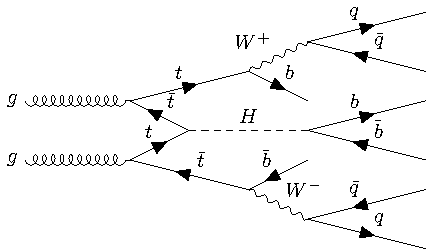
\includegraphics[width=\textwidth]{Feynman/tth.pdf}
        \caption{Particle interactions}
        \label{fig:feynman}
    \end{subfigure}
    \begin{subfigure}[b]{0.45\textwidth}
        \centering
        \includegraphics[width=\textwidth]{Figures/graph_networks/RifampiciN_Structure.pdf}
        \caption{Chemical compounds}
        \label{fig:chemical}
    \end{subfigure}
    \begin{subfigure}[b]{0.45\textwidth}
        \centering
        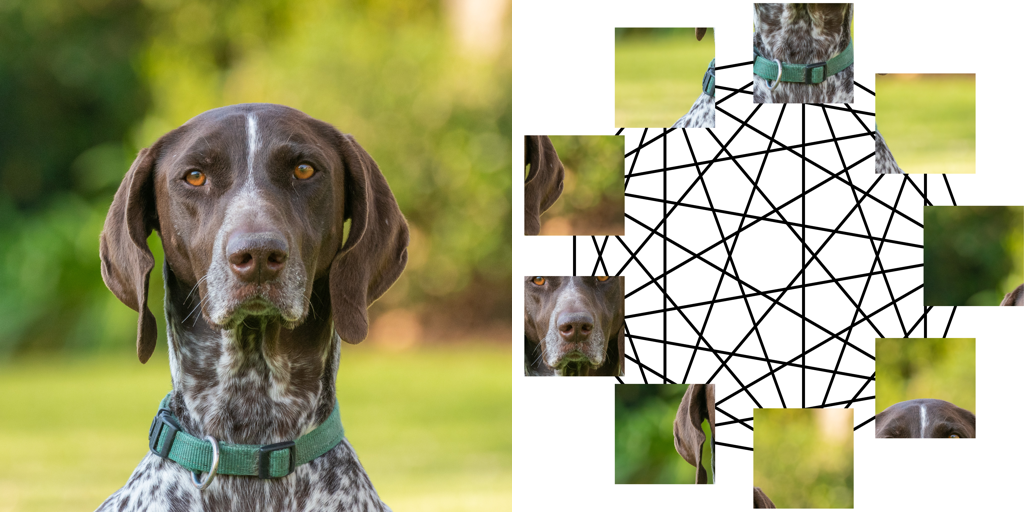
\includegraphics[width=\textwidth]{Figures/graph_networks/patched_image.png}
        \caption{Images (patched)}
        \label{fig:dog}
    \end{subfigure}
    \begin{subfigure}[b]{0.45\textwidth}
        \centering
        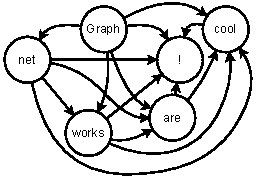
\includegraphics[width=0.8\textwidth]{Figures/graph_networks/text.pdf}
        \caption{Language (tokenized)}
        \label{fig:text}
    \end{subfigure}
    \caption{Examples of data that can be represented as graphs.}
    \label{fig:graph_examples}
\end{figure}

\subsection{Interconnectivity}

When constructing a graph representation it is crucial to consider its interconnectivity; which pairs of nodes have edges between them.
GNNs propagate information along edges, so the structure of the graph can have a significant impact on the model's performance.
Interconnectivity is closely tied to two key issues in GNNs: over-squashing~\cite{OverSquashing} and the over-smoothing~\cite{OverSmoothing}.

The inductive bias of locality can be imposed in a graph by only connecting nodes close to each other in some metric space.
However, limiting the connections of each node to its local neighbourhood can also mean that long term dependencies may get lost.
This is because multiple rounds of message passing are required to propagate information between distant nodes as shown in \Cref{fig:neighbours}.
With each round, exponentially more neighbouring nodes need to project information into a fixed-size vectors leading to an over-squashing of information.
It is exacerbated by bottlenecks in the graph structure as shown in \Cref{fig:bottleneck}, where the information between nodes $\x_i$ and $\x_j$ must pass along a single edge which must also carry information from their respective neighbourhoods.

There are many proposed solutions to the over-squashing problem.
The inclusion of global features in the graph may help model long range dependencies, however the size of the global tensor would need to scale with the cardinality of the set.
Another solution is to simply increase the number of edges in the graph, allowing for more direct paths between nodes.
This is known as graph rewiring and can be focussed around bottlenecks in the graph, identified by regions of low Forman curvature~\cite{UnderstandingOversquashingBottlenecks}.

There are however downsides to graph rewiring.
First, it means loosening the locality inductive bias.
The extreme case of this is a fully connected graph, where edges exist between all pairs of nodes in both directions and locality is completely lost.
Secondly, is that it exacerbates the other issue with GNNs, over-smoothing.
This refers to the phenomenon where all node features across the graph converge towards the same constant value as the number of message passing steps increases.
This one of the reasons that the depth of most GNNs is notably shallower than other deep learning models, as with every round of message passing each node aggregates information from its neighbours, diluting the original information.
There are many proposed solutions to this issue, such as residual connections~\cite{DeepGCNs}, normalization layers~\cite{PairNorm}, and regularization~\cite{DirichletEnergyConstrained}.
Finally, there is a computational cost to increasing the number of edges in the graph.
Many models are looking to find way to minimize the interconnectivity while preserving model quality~\cite{GeneratingLongSequences}.

\subsubsection{When is an Inductive Bias Holding You Back?}

As previously mentioned, one of the key inductive biases leading to the success of CNNs is the locality of the convolutional kernel.
However, the state-of-the-art models in computer vision are GNNs operating on fully connected graphs of image patches~\cite{VisionTransformer}, demonstrating that locality in images is not always useful.
This makes intuitive sense, as the content of an image is not always localized; objects can be spread out across multiple patches, and they may be obscured, only visible in physically separated regions of the image.

This extends to the example of the chemical compound in \Cref{fig:chemical}.
In this model the edges are defined by the chemical bonds between the atoms.
However, long range dependencies do exist in chemistry.
The function of one part of a protein may be altered by the presence of a ligand on the other side of the molecule.
Constraining the message passing graph to match the physical graph may limit the model from learning these relationships.

The GNNs that work well in these cases are equipped with all the tools needed to combat over-smoothing mentioned in the previous section, as well as the attention mechanism~\cite{Attention}.
Attention refers the learnable process of weighting the incoming messages before aggregation.
It allows the GNN to ``pay more attention'' to specific connections within the graph.

This raises the point that if we have enough data and a large enough model, enforcing what relationships are important may not be necessary, and it is better to let the model learn these rules itself.
It also raises whether the message passing graph and the input data graph should be tied together at all.
Models such as the perceiver~\cite{Perceiver} project input information onto a completely different latent graph for message passing and recent work for GNNs in computer vision has shown that they require extra, fully learnable nodes not tied to any image patch~\cite{VisionTransformersNeed}.

\begin{figure}
    \centering
    \begin{subfigure}[b]{0.3\textwidth}
        \centering
        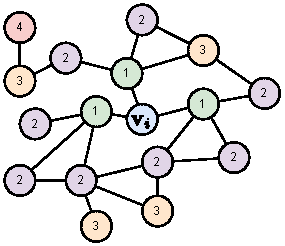
\includegraphics[width=\textwidth]{Figures/graph_networks/neighbours.pdf}
        \caption{}
        \label{fig:neighbours}
    \end{subfigure}
    \begin{subfigure}[b]{0.3\textwidth}
        \centering
        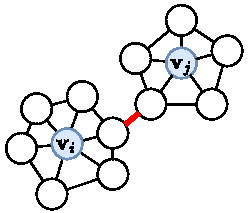
\includegraphics[width=\textwidth]{Figures/graph_networks/bottleneck.pdf}
        \caption{}
        \label{fig:bottleneck}
    \end{subfigure}
    \caption{\subref{fig:neighbours} The locality of information flow in a graph. On each node is the number of message passing steps required to propagate information to the node $\vert_i$.\ \subref{fig:bottleneck} A graph with a bottleneck. Information being passed between nodes $\vert_i$ and $\vert_j$ must pass through a single edge shared by each of the sub-clusters.}
    \label{fig:over_squashing}
\end{figure}

\section{The Graph Network Block}
\label{sec:gn_block}

The Graph Network Block (GN Block)~\cite{RelationalInductiveBiases} is a useful building block for constructing deep learning models that operate on graph-structured data.
It offers a framework that generalizes to many other existing graph-based models, such as graph convolutional networks (GCNs)~\cite{GCN}, graph attention networks (GATs)~\cite{GraphAttentionNetworks}, deep sets~\cite{DeepSets}, and even transformers~\cite{Attention}.
A GN Block is defined as a series of operations that update the node, edge, and global attributes via facilitating the exchange and aggregation of information according to the structure of the graph.
The GN Block does not change the cardinality of the features present, only updating their attributes,
\begin{equation}
    \text{GN}(\mathcal{N}, \mathcal{E}, \u) = (\mathcal{N}', \mathcal{E}', \u').
\end{equation}
The GN block is composed of three sub-blocks involving three update functions, $\phi^x$, $\phi^e$, and $\phi^u$, and three aggregation functions, $\rho^{e \to x}$, $\rho^{e \to u}$, and $\rho^{x \to u}$.
Given an input graph $\mathcal{G} = (\mathcal{N}, \mathcal{E}, \u)$ the GN Block proceeds as follows.

\begin{enumerate}
    \item \textbf{Edge Block:} The edges are updated using the current edge attributes, the attributes of the sender and receiver nodes, and the global attribute.
    \begin{equation}
        \edge_k' = \phi^e(\edge_k, \x_{s_k}, \x_{r_k}, \u).
    \end{equation}
    All edges throughout the graph are updated in this manor and this step can be executed in parallel.
    The updated edges $\edge_k'$ can be thought of as the message being passed from the sender to the receiver.
    \item \textbf{Node Block:} Incoming edge information is aggregated for each node.
    For node with index $i$, this is represented by the set $E_i$.
    \begin{equation}
        \bar\edge_i = \rho^{e \to x}(E_i) = \rho^{e \to x}\left(\{(\edge_k', r_k, s_k) | r_k = i\}\right)
    \end{equation}
    All nodes are then updated using its current attributes, the aggregated edge information, and the global attribute.
    Updating the nodes using incoming information is called message passing.
    \begin{equation}
        \x_i' = \phi^x(\bar\edge_i, \x_i, \u).
    \end{equation}
    \item \textbf{Global Block:} All edge information and node information across the graph is aggregated,
    \begin{alignat}{2}
        \bar\x &= \rho^{x \to u}(\mathcal{N}') &&= \rho^{x \to u}(\{\x_i\}_{i=1}^{N}) \\
        \bar\edge &= \rho^{e \to u}(\mathcal{E}') &&= \rho^{e \to u}(\{\edge_k'\}_{k=1}^{N^e}),
    \end{alignat}
    and used to update the global attribute,
    \begin{equation}
        \u' = \phi^u( \bar\edge, \bar\x, \u).
    \end{equation}
\end{enumerate}

The GN Block describes a basic graph to graph transformation which can be composed to form a deeper model.
To make the block learnable, each of the update or aggregation functions may be parameterized by a separate neural network.
The only requirement for any of the aggregation functions is that they are permutation invariant and may accept a variable number of arguments.
This structure also lends itself to the different types of tasks performed on graph type data.
For example, the final GN Block in the stack may only contain an edge block for an edge-level task.

It is important to investigate exactly what inductive biases are being imposed by the GN Block.
First, it is clear that the updates to the graph do not depend on the order of the nodes.
Formally, the node and edge updates $(\mathcal{N}, \mathcal{E}) \rightarrow (\mathcal{N}', \mathcal{E}')$ are permutation equivariant to the node set, and the global update $U \rightarrow U'$ is permutation invariant.
The GN Block applies the same update and aggregation functions to all nodes and edges in the graph.
This reflects the relational inductive bias which seeks to learn general rules that apply to all entities in the system while also adhering to the equivalence of the elements within the set.
Furthermore, as the GN Block only prescribes the rules for how the features of a graph are updated, it is agnostic to the structure and size of the input graph.
This allows the same model to be applied to input sets with varying cardinality or connectivity.
This is a crucial feature for many applications, such as in collider physics where the number of particles in an event can vary.
Finally, information flow between elements of the set can follow two paths.
Either, the information propagates along the edges of the graph, or it is aggregated into the global attribute, then redistributed to the nodes.
This allows for the model to learn both local and long-range interactions.

Almost all GNNs variants facilitate message passing can be thought of as some specialization of the GN Block depending on the forms of the $\phi$ and $\rho$ functions and the existence of edge, node, and global features.
A full GN Block is shown in \Cref{fig:full_gn_block}.
A basic implementation, where all graph attributes are tensors, can be done using MLPs for each of the update functions, and summation for the aggregation functions.
This creates the update shown in \Cref{alg:gn_block}, where the square brackets denote tensor concatenation.
Even the deep set, which has no pairwise interactions between the nodes can be seen as a reduced form of a GN Block, as shown in \Cref{fig:deep_set}.
Here the operations are simply,
\begin{align}
    \x_i' &= \text{MLP}_v\left(\left[\x_i, \u\right]\right),\\
    \u' &= \text{MLP}_u\left(\left[\sum_{i} \x_i', \u\right]\right).
\end{align}

\begin{algorithm}
    \caption{Basic GN Block using MLPs}
    \label{alg:gn_block}
    \begin{algorithmic}[1]
        \State \textbf{Input:} Graph attributes $\mathcal{G} = (\mathcal{N}, \mathcal{E}, \u)$
        \State \textbf{Output:} Updated graph attributes $\mathcal{G}' = (\mathcal{N}', \mathcal{E}', \u')$
        \For{each edge $\edge_k$ in $\mathcal{E}$}
            \State $\edge_k' \gets \text{MLP}_e([\edge_k, \x_{s_k}, \x_{r_k}, \u])$ \Comment{update edge features}
        \EndFor
        \For{each node $\x_i$ in $\mathcal{N}$}
            \State $\mathbf{\bar\edge}_i \gets \sum_{k: r_k = i} \edge_k'$ \Comment{aggregate incoming information per node}
            \State $\x_i' \gets \text{MLP}_v([\mathbf{\bar\edge}_i, \x_i, \u])$ \Comment{update node features}
        \EndFor
        \State $\mathbf{\bar{x}} \gets \sum_{i} \x_i'$ \Comment{aggregate features across the graph}
        \State $\mathbf{\bar\edge} \gets \sum_{k} \edge_k'$
        \State $\u' \gets \text{MLP}_u([\mathbf{\bar\edge}, \mathbf{\bar{x}}, \u])$ \Comment{update global features}
    \end{algorithmic}
\end{algorithm}

\begin{figure}
    \centering
    \begin{subfigure}[b]{0.49\textwidth}
        \centering
        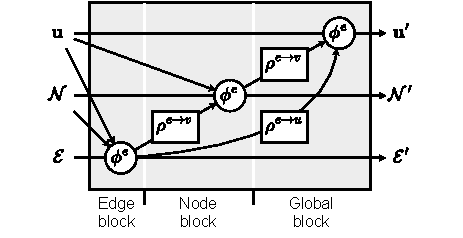
\includegraphics[width=\textwidth]{Figures/graph_networks/full_gn.pdf}
        \caption{Full GN Block}
        \label{fig:full_gn_block}
    \end{subfigure}
    \begin{subfigure}[b]{0.49\textwidth}
        \centering
        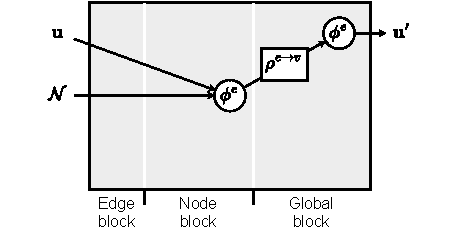
\includegraphics[width=\textwidth]{Figures/graph_networks/deepset.pdf}
        \caption{Deep Set}
        \label{fig:deep_set}
    \end{subfigure}
    \caption{Examples of different GN Block implementations \subref{fig:full_gn_block} A full GN Block has persistent edge and global features. \subref{fig:deep_set} A deep set only applies pooling to the node features to produce a global feature. Adapted from \textcite{RelationalInductiveBiases}.}
\end{figure}

\section{Transformers are Graph Networks}
\label{sec:transformers}

It is hard to overstate the impact of the transformer model~\cite{Attention} on deep learning.
Originally designed for NLP sequence-to-sequence tasks, transformers far surpassed the performance of all previous models, so much so that research in other sequence-based models, such as recursive neural networks, almost ceased entirely.
They also marked a massive leap in commercializing deep learning for NLP.
Starting in 2018, OpenAI began releasing the GPT~\cite{GPT} series of transformer models, arguably triggering a boom around large language models that continues to this day.
In 2019, Google announced that they were using the transformer-based BERT model~\cite{BERT} to power their search engine and transformers for their translation service.
In 2020, transformers were adapted to work on image data~\cite{VisionTransformer}, marking the point where transformers took the crown in computer vision benchmarks from CNNs as shown in \Cref{fig:benchmarks}.
Even image generation tasks that used to be dominated by UNets~\cite{Unet, DiffusionBeatsGANS} are now being performed by transformers~\cite{DIT, SD3}.
Transformers have become so ubiquitous that they are now considered the default choice for many deep learning tasks, regardless of the data type.

There are many variants for the transformer model, but they all share the same basic features.
Contrary to popular belief, these models do not natively run on sequences but on sets, and must be adapted to work on data with an inherent order.
We will focus on two main types of transformers, the transformer encoder and the transformer decoder.
The transformer encoder (TE) is a variant of the GN Block called a non-local neural network (NLNN)~\cite{NonlocalNeuralNetworks} as shown in \Cref{fig:transformer}.
This function operates on a pure set, with no persistent edge or global features.
It involves and message passing step equipped with an attention mechanism, followed by a node update step using an MLP\@.

The jargon of transformers differs slightly from that of GNNs.
Nodes are called tokens in many research papers on transformers.
The term attention is also used more broadly in transformers, not just referring to the means of weighting and aggregation, it is sometimes used to refer to the entire message passing step.
Furthermore, saying that a node attends to another is equivalent to saying that the node receives a message from another.
The adjacency matrix in a graph is also called the attention mask in a transformer.

\begin{figure}[h]
    \centering
    \begin{subfigure}[b]{0.49\textwidth}
        \centering
        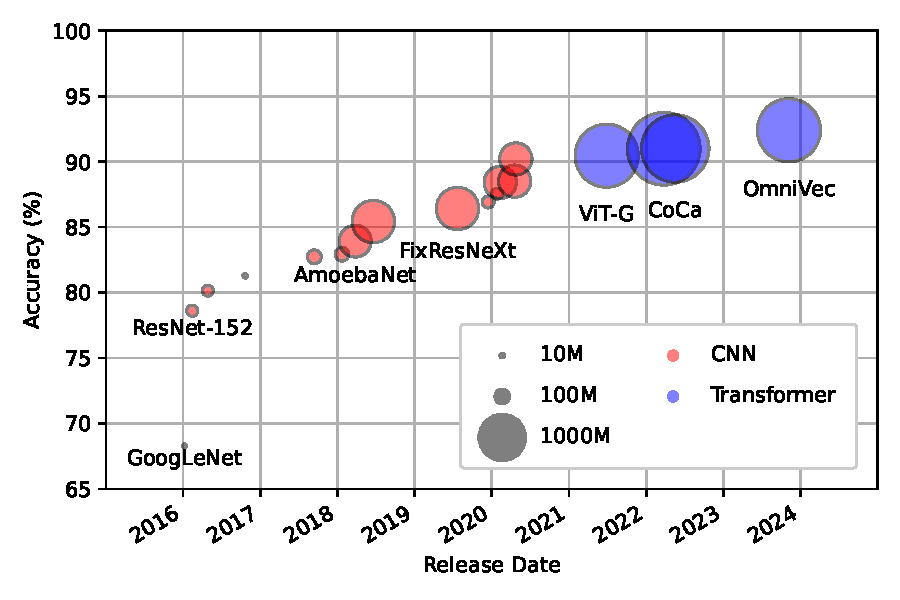
\includegraphics[width=\textwidth]{Figures/graph_networks/imagenet.pdf}
        \caption{}
        \label{fig:imagenet}
    \end{subfigure}
    \hfill
    \begin{subfigure}[b]{0.49\textwidth}
        \centering
        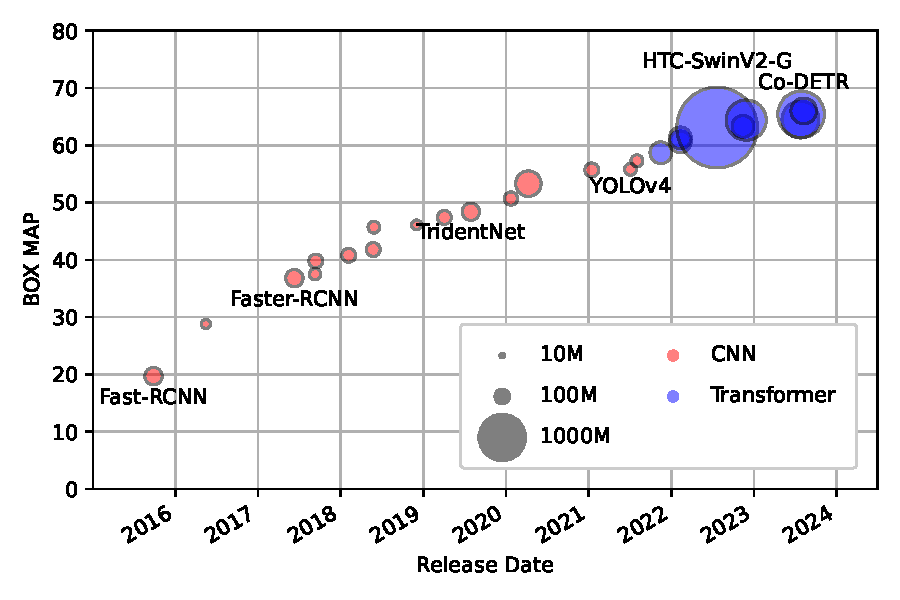
\includegraphics[width=\textwidth]{Figures/graph_networks/coco.pdf}
        \caption{}
        \label{fig:coco}
    \end{subfigure}
    \caption{Evolution of the state-of-the-art models in two common computer vision benchmarks~\cite{paperswithcode}. The size of the markers corresponds to the number of trainable parameters in the model. \subref{fig:imagenet} Accuracy on the ImageNet classification benchmark. \subref{fig:coco} Bounding box mean average precision (BOX MAP) the COCO object detection benchmark.}
    \label{fig:benchmarks}
\end{figure}

\begin{figure}
    \centering
    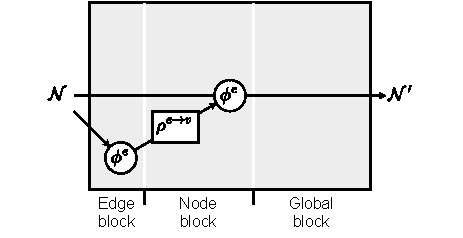
\includegraphics[width=0.49\textwidth]{Figures/graph_networks/nonlocal.pdf}
    \caption{NLNN / Transformer Encoder}
    \label{fig:transformer}
\end{figure}

\subsection{Transformer Attention is Just Message Passing}
\label{sec:attention}

There are many of ways to parameterize the message passing step in a GNN, and the one used in the transformer is the scaled dot-product attention (SDPA).
In SDPA, the message passed between nodes is a linear projection of the sender node attributes.
This means that each node sends out the same message to all of its neighbours called its \textit{value}, $\vert_{i} = \mathbf{W}^v \x_i$.
The message weight is based on a dot product between additional linear projections of the sender node, called they key \textit{key} $\k_{i} = \mathbf{W}^k \x_i$, and the receiver node, called the \textit{query} $\q_{j} = \mathbf{W}^q \x_j$.
Aggregation is simply a weighted mean of the incoming messages, where a softmax operation is applied to the attention logits to ensure that they sum to one.
To prevent the gradients from exploding, the attention logits are scaled by the square root of the dimensionality of the key and value tensors $d_k$.

In the framing of the GN Block, SDPA has the edge update is factorized into a tuple containing a scalar expressing the message weight $\alpha_k'(\x_{s_k}, \x_{r_k})$ and a vector function for calculating the message content $\mathbf{v}_k'(\x_{s_k})$.
Only $\alpha_k'$ depends on the pairwise interaction of both the sender and receiver nodes.
The pooling operation $\rho^{e \to x}$ normalizes over the receiver weights before aggregating the messages.
The block can be written as,
\begin{equation}
    \begin{aligned}
        \edge_k' &= \phi^e(\edge_k, \x_{s_k}, \x_{r_k}, \u)
        = ( a_k', \mathbf{v}_k' ) \\
        &= \left( \exp \left( \frac{1}{d_k} \mathbf{W}^q \x_{s_k} \cdot \mathbf{W}^k \x_{r_k} \right), \mathbf{W}^v \x_{s_k} \right), \\
        \mathbf{\bar\edge}_i &= \rho^{e \to x}(E_i) \\
       &= \frac{\sum_{k: r_k = i} a_k' \mathbf{v}_k'}{\sum_{k: r_k = i} a_k'},
    \end{aligned}
\end{equation}
for learnable weight matrices $\mathbf{W}^k \in \mathbb{R}^{d \times d_k}$, $\mathbf{W}^q \times \mathbb{R}^{d \times d_k}$, and $\mathbf{W}^x \in \mathbb{R}^{d \times d_v}$.

When using real values tensor representations, this operation can be done efficiently for all nodes in parallel using basic matrix operations.
Furthermore, it allows us to extend to two forms, self-attention and cross-attention, both expressible by the following equation,
\begin{equation}
    \label{eq:attention}
    \begin{aligned}
        \text{Attention}(\X_R, \X_S)
        &= \text{softmax}\left(\frac{(\X_S \mathbf{W}^q) (\X_R \mathbf{W}^k)^T}{d_k} + \mathbf{B}\right) \X_S \mathbf{W}^v, \\
        &= \text{softmax}\left(\frac{\mathbf{Q} \mathbf{K}^T}{d_k} + \mathbf{B}\right) \mathbf{V}.
    \end{aligned}
    \end{equation}
In this expression we distinguish between the tensor representing the sender nodes $\X_S \in \mathbb{R}^{N_S \times d}$ and the receiver nodes $\X_R \in \mathbb{R}^{N_R \times d}$.
Self-attention is where the sender and receiver set are the same $\X_S = \X_R$.
This is the standard message passing operation between nodes in a graph.
Cross-attention is where the sender set and receiver set are different $\X_S \neq \X_R$.
This operation is permutation invariant with respect to $\X_S$ and equivariant with respect to $\X_R$.
As shown by \Cref{fig:bipartite}, one can interpret this as the construction of a one-way bipartite graph between two sets, where all nodes in $\X_S$ send messages to all nodes in $\X_R$.
Note that the cardinality of the sender and receiver sets do not need to be the same.
Cross-attention is a powerful tool to condition one set on another and is used in many sequence to sequence tasks, from translation, to image captioning, and text-to-image generation.
Finally, the bias term $\mathbf{B}$ is a matrix of shape $(N_R, N_S)$ which can be used to focus or ignore certain pairs of nodes.

\begin{figure}
    \centering
    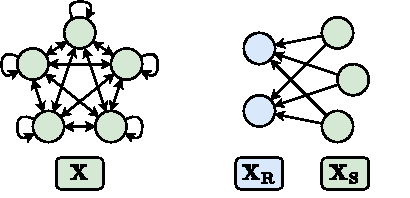
\includegraphics[width=0.5\textwidth]{Figures/graph_networks/bipartite.pdf}
    \caption{(left) Self-attention is standard message passing between all nodes in a graph. (right) Cross-attention creates a one-way bipartite graph between two sets of nodes.}
    \label{fig:bipartite}
\end{figure}

Transformers typically extend this operation to multi-headed attention (MHA), as shown in \Cref{fig:mha}.
This is where SDPA is performed $H$ times in parallel with different matrices $\mathbf{W}^q$, $\mathbf{W}^k$, $\mathbf{W}^v$, and $\mathbf{B}$.
The output of each head is concatenated and then mixed using a final linear layer,
\begin{equation}
    \begin{aligned}
    & \text{Head}_1 = \text{Attention}(\X_R, \X_S), \\
    & \text{Head}_2 = \text{Attention}(\X_R, \X_S), \\
    & \ldots, \\
    & \text{Head}_H = \text{Attention}(\X_R, \X_S), \\
    \vphantom{x} \\
    & \text{MHA}(\X_R, \X_S) = \text{Concat}(\text{Head}_1, \ldots, \text{Head}_H) \mathbf{W}^o.
    \end{aligned}
\end{equation}
In MHA, many types of messages are passed between the nodes and one can think of this as constructing a multi-graph on the set.
Both self- and cross-attention can be multi-headed where multi-headed self-attention (MHSA) is defined as $\text{MHSA}(\X) = \text{MHA}(\X, \X)$.

\begin{figure}
    \centering
    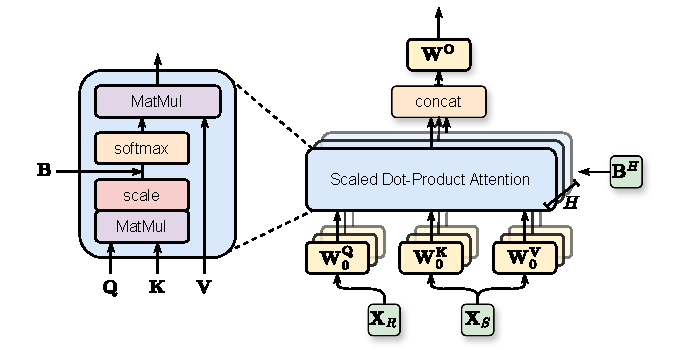
\includegraphics[width=0.8\textwidth]{Figures/graph_networks/mha.pdf}
    \caption{Multi-headed attention can be thought of as constructing a multi-graph with different edge types.}
    \label{fig:mha}
\end{figure}

\subsubsection{Implementing Multi-Headed Attention}

The dot product in the SDPA layer necessitates that the dimensions of key and query tensors are equal.
Additionally, the majority of SDPA implementations do not resize, resulting in $\mathbf{Q}$, $\mathbf{K}$, and $\mathbf{V}$ all having the same shape.
When extending to MHA, it is standard to split the dimensionality equally by the number of heads $H$.
This means that a single MHA function is typically parameterized by four square matrices corresponding to $4d^2$ learnable parameters with the number of heads $H$ being the sole hyperparameter of the block.

To enhance the model's expressivity, one can replace linear projections with affine transformations by including bias terms. However, it is important to note that the bias of the key operation is entirely redundant~\cite{RoleBiasTerms}.

Key to the success of transformers is the ease of implementation.
While many variants of GN Block block variants require custom libraries and are challenging to implement from scratch, MHA can be implemented in PyTorch using standard linear algebra operations, as demonstrated in \Cref{code:attention}.
All heads are computed in parallel using smart reshaping of the tensors.
This significantly simplifies the process of designing, building, testing, and exporting models.

While the message passing operation is considerably simpler than using MLPs for each stage as described in~\Cref{alg:gn_block}, it is possible to enhance the model's expressivity by scaling either the model dimension or the number of heads.
Contrary to popular belief, self-attention with these mechanisms does not require $O(N^2)$ memory complexity. There are algorithms available that achieve this without needing to manifest the full attention matrix~\cite{SelfattentionDoesNot, FlashAttentionFastMemoryEfficient}.

\begin{figure}
    \centering
    \scriptsize
    \begin{minted}{python}
    class Attention(nn.Module):
        def __init__(self, dim: int, num_heads: int):
            super().__init__()
            self.NH = num_heads
            self.HD = dim // num_heads
            self.scale = self.HD**-0.5
            self.wk = nn.Linear(dim, dim)
            self.wq = nn.Linear(dim, dim)
            self.wv = nn.Linear(dim, dim)
            self.wo = nn.Linear(dim, dim)

        def forward(self, xr: T.Tensor, xs: T.Tensor, bias: T.Tensor | int = 0) -> T.Tensor:
            q, k, v = self.wq(xs), self.wk(xr), self.wv(xs)              # project
            shape = (xr.shape[0], -1, self.NH, self.HD)                  # split heads
            q, k, v = (t.view(shape).transpose(1, 2) for t in (q, k, v))
            attn = (q @ k.transpose(-2, -1))                             # attention weight
            attn = (attn * self.scale + bias).softmax(dim=-1)
            x = attn @ v                                                 # aggregate
            x = x.transpose(1, 2).reshape(B, N, D)                       # mix heads
            return self.wo(x)
    \end{minted}
    \caption{A simple implementation of a multi-headed attention block in PyTorch.}
    \label{code:attention}
\end{figure}

% \subsubsection{Efficiency of Scaled Dot-Product Attention}

% SDPA stands out as an exceptionally efficient method for expressive message passing in fully connected graphs.
% To illustrate this, we can start by examining the simplest GNN variant, the GCN~\cite{GCN}, and identify its limitations.

% A single GCN layer, without normalization factors, can be expressed as,
% \begin{equation}
%     \begin{aligned}
%     \edge_k' &= \mathbf{W} \x_{s_k}, \\
%     \x_i' &= \sum_{k:r_k=i} \edge_k',
%     \end{aligned}
% \end{equation}
% for a single learnable weight matrix $\mathbf{W}$.
% Let us consider the shapes of the tensors in this operation.
% Representing the set of nodes as a real-valued tensor $\mathbf{X}$ of shape $(N, d)$, the operation can be performed using a matrix multiplication $\mathbf{W}: (N, d) \rightarrow (N, d)$, followed by a sum.

% In a fully connected graph, after one update step, every node would contain the same information, leading to an extreme case of over-smoothing.

% To avoid this over-smoothing, each message must be unique for each node pair.
% Thus, the challenge becomes finding the most efficient way to parameterize messages such that the output of the message constructing process is a tensor with shape $(N, N, d)$.
% Here we assume that the dimension of the nodes and the edges is the same.
% The first dimension in this tensor represents sender nodes, and the second dimension represents receiver nodes.
% The aggregation operation then acts over the first dimension to produce a tensor of shape $(N, d)$,
% \begin{align}
%     \text{construct method}: (N, d) & \rightarrow (N, N, d) \\
%     \text{aggregate}: (N, N, d) & \rightarrow (N, d).
% \end{align}

% The basic GN Block in \Cref{alg:gn_block} does this by concatenating the sender and receiver node attributes before passing them through an MLP\@.
% The operations and dimensions of the tensors of such a block are,
% \begin{align}
%     \text{concatenate}: (N, d) & \rightarrow (N, N, 2d) \\
%     \text{MLP}: (N, N, 2d) & \rightarrow (N, N, d) \\
%     \text{sum}: (N, N, d) & \rightarrow (N, d)
% \end{align}
% This meets the criteria for a highly expressive message passing operation, but it is not the most efficient, since a large tensor of shape $(N, N, 2d)$ is created and needs to be passed through a learnable operation, here an MLP.
% With very large graphs, we would like to avoid the construction of tensors with $O(N^2)$ elements.
% One way to mitigate this is to factorize the step into two learnable components, one to calculate the message weight (attention) and one to calculate the message content (value).

% Only one of these needs to be unique for each pairing and since the weight is a scalar and the content is a vector, it is much more efficient to allow the content to be degenerate.
% This is exactly the approach of GATs~\cite{GAT}, which perform the update,
% \begin{align}
%     \mathbf{W_1}&: (N, D)  \rightarrow (N, D) \\
%     \text{concatenate}&: (N, D)  \rightarrow (N, N, 2D) \\
%     \mathbf{W_2}&: (N, N, 2D)  \rightarrow (N, N) \\
%     \text{matrix multiply}&: (N, N), (N, D)  \rightarrow (N, D)
% \end{align}
% However, there is still the issue that this input and output of the learnable layers are $O(N^2)$.

% The $(N, N)$ matrix of attention weights needs to be learnable from the original $(N, D)$ node attributes and must be allowed to be unique for each pairing.
% Therefore, there must be a distinction between the sender and receiver nodes, this makes the required map $a: (N, D), (N, D) \rightarrow (N, N)$.
% There are few operations that can achieve this, and none so efficient as a dot product.
% Using linear projections for the initial embeddings means that the K, Q, V tensors can be computed in parallel.
% \begin{align}
%     \mathbf{W}: (N, D) & \rightarrow (N, 3D) \\
%     \text{split}: (N, 3D) & \rightarrow (N, D), (N, D), (N, D) \\
%     \text{scale-dot-softmax}: (N, D), (N, D) & \rightarrow (N, N) \\
%     \text{matrix multiply}: (N, N), (N, D) & \rightarrow (N, D)
% \end{align}
% While the other parts of the update do require $O(N^2)$ operations, crucially the input and output of the learnable layers dependent is only $O(N)$.

% The argument made here is that one will struggle to find a more simple and efficient way to parameterize the message passing step in a GNN that does not lead to over-smoothing when fully connected.
% The philosophy of the transformer is similar to the philosophy of composing MLPs from linear layers, in that the composition of simple, highly parameterized functions, is what provides expressivity.
% By and large the most complex component of the operation is the softmax function, but there exist algorithms to calculate this online without having to express the full attention matrix~\citetemp{FlashAttention}.
% Contrary to popular claims, self-attention with these mechanisms is non $O(N^2)$ in memory complexity~\citetemp{MemoryComplexity}.
% Some more recent models large models have even done away with the softmax, citing better performance beyond a certain model scale~\citetemp{Reformer, LinearAttetnion}.

\subsection{Transformer Variants}
\label{sec:transformer_variants}

There are numerous transformer variants, too many to cover in this thesis.
Common similarities exist among them, though terminology can be ambiguous and overlapping.
A single transformer block generally includes two types of sub-blocks: MHA for message passing and FFN/MLP layers for the node update.
These sub-blocks combine and repeat to form the larger transformer block.
MHA layers can be configured as self-attention or cross-attention, and are typically stacked with FFN layers in series~\cite{Attention}, but sometimes in parallel~\cite{Palm}.
Another distinguishing feature is the use of residual connections and normalization layers with various configuration options to stabilize training and prevent over-smoothing
Due to the wide range of transformer variants, empirical performance is often the guide for best practices.

Most transformer layers use an MLP with a single hidden layer that expands the node attributes' dimensionality by a factor of $M$.
However, modern transformers use Gated Linear Units (GLU)~\cite{GLU}, a network layer involving the element-wise multiplication of two linear projections, one of which is activated~\cite{SwiGLU},
\begin{equation}
    \text{FFN}_\text{SwiGLU}(\x_i) = \mathbf{W}_3(\text{Swish}(\mathbf{W}_1 \x_i + \mathbf{b}_1) \otimes (\mathbf{W}_2 \x_i + \mathbf{b}_2)) + \mathbf{b}_3.
\end{equation}
Many transformers also use the mixture-of-experts approach, where there exist many FFN layers, each with different parameters, and a gating mechanism to direct certain nodes to certain experts~\cite{MOE}.
Notably, while attention mechanisms are key to transformers' success, the majority of parameters are in these node update layers.

Residual connections are typically used to circumvent each sub-block.
The original transformer used a PostNorm configuration, where layer normalizations were applied after each residual connection~\cite{Attention}.
This was found to excessively squash the signal; therefore, contemporary transformers often utilize the PreNorm configuration~\cite{PreLN}.
Extra normalization within the sub-blocks is also common.

\subsubsection{Transformer Encoder}

A single PreNorm TE Block is shown in \Cref{fig:transformer_blocks}.
The update is given by,
\begin{equation}
\begin{aligned}
    \X & \leftarrow \X + \text{MSHA}(L_\text{norm}(\X)), \\
    \X & \leftarrow \X + \text{FFN}(L_\text{norm}(\X)).
\end{aligned}
\end{equation}
A full TE is composed of many TE Blocks stacked in series forming a permutation equivariant set to set transformation.
For many tasks, the TE is the main feature extractor.

\subsubsection{Transformer Decoder}

To condition the update of one set on another, a cross-attention (CA) block, can be utilized.
For a more expressive operation, the layer can include both self-attention and cross-attention, creating a transformer decoder (TD) block, as shown in \Cref{fig:transformer_blocks}.
The update of a TD block is written as,
\begin{equation}
\begin{aligned}
    \X_R & \leftarrow \X_R + \text{MHSA}(L_\text{norm}(\X_R)), \\
    \X_R & \leftarrow \X_R + \text{MHA}(L_\text{norm}(\X_R), \X_S), \\
    \X_R & \leftarrow \X_R + \text{FFN}(L_\text{norm}(\X_R)).
\end{aligned}
\end{equation}
The TE and TD are typically combined to create a set-to-set transformation that first extracts features from the input set, and the conditions the output set on these features.
This set-to-set transformation is the basis of many generative of sequence-to-sequence models.

\begin{figure}
    \centering
    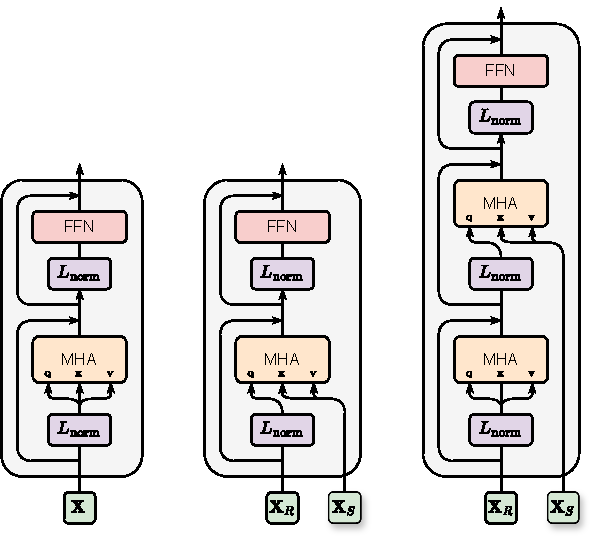
\includegraphics[width=0.7\textwidth]{Figures/graph_networks/transformer_variants.pdf}
    \caption{Some common transformer variants. (left) Transformer Encoder (TE) block. (center) Cross-Attention (CA) block. (right) Transformer Decoder (TD) block.}
    \label{fig:transformer_blocks}
\end{figure}

\subsection{Edge Attributes, Biases, and Sequences}
\label{sec:edge_biases_sequences}

When viewing the transformer as a GNN, the inclusion of edge information becomes intuitive.
For message passing on a single graph, if not represented sparsely, edge information is stored in a tensor $\edge \in \mathbb{R}^{N \times N \times d_e}$.
In the SDPA operation in \cref{eq:attention}, the attention matrix defined by,
\begin{equation}
    \mathbf{A} = \text{softmax}\left( \frac{\mathbf{Q} \mathbf{K}^T}{d_k} + \mathbf{B} \right),
\end{equation}
which has the shape $(N, N)$ for self-attention.
Extending this to MHA it gains an extra dimension $(N, N, H)$ aligning with the required shape of the edge tensor and making it the only valid candidate in the entire operation.
The query and key tensors $\mathbf{Q}$ and $\mathbf{K}$ stem from projections of the input, but $\mathbf{B}$ must have shape which is at least broadcastable to $(N, N, H)$.
Consequently, edge information can be integrated into a transformer through the bias term in the attention operation, a practice used in various scenarios.

The Particle Transformer (ParT)~\cite{ParticleTransformerJet} uses a TE to embed a set of particles, defined by their kinematics.
For each pair of particles, specific edge features are constructed using Lund Plane variables~\cite{LundJetPlane}.
The model uses an MLP to embed these edge features into a tensor of shape $(N, N, H)$, which becomes the attention bias in each of the TE Blocks.

The bias tensor is commonly set to negative infinity for specific node pairs and all heads, forcing the attention weight to zero after the softmax operation and eliminating the message weight. This allows the transformer to function on non-fully connected graphs without changing any of the underlying matrix operations.
It is also one of the main mechanisms for adapting the transformer to work on sequences, where the nodes are presented in a specific order.
By configuring the bias matrix as a lower triangular matrix with above-diagonal entries set to negative infinity, each node receives messages only from preceding nodes.
This technique, known as a causal masking, is used extensively in generative models as it lends itself to autoregressive sampling.
Causal masking allows for highly efficient training, as each stage of the autoregressive generation can be computed in a single forward pass.
Although generation requires sequential model execution, the training speed-up is a substantial benefit.
Many sequence generating models are called ``decoder only'', however in the presented framework, these models are TE models with a causal attention mask.

While a causal mask suffices for a transformer to grasp order~\cite{TransformerLanguageModels}, it is often complemented by \textit{positional encoding}.
Absolute positional encoding (APE) integrates sequence positions into node attributes.
A unique tensor $\mathbf{p}_i \in \mathbb{R}^{d}$ is constructed for each possible observed position $i$ and is added to the node attributes before the first transformer block, $\x_i \leftarrow \x_i + \mathbf{p}_i$.
Originally, fixed sinusoidal functions of varying frequencies encoded these positions, but recent models make $\mathbf{p}_i$ fully learnable~\cite{GPT}.
In images, APE, often termed spatial encoding, involves encoding and adding the 2D coordinates of a patch to its representation~\cite{VisionTransformer}.

APE is limited in capturing relative positions, necessitating the use of relative positional encoding (RPE)~\cite{SelfAttentionRelativePosition}.
RPE biases the attention matrix, serving as edge information, with various implementations.
$B$ can be parameterized as a learnable Toeplitz matrix, ALiBi~\cite{ALIBI} fixes the elements of this matrix to be simply $B_{ij} = m\times(i - j)$, for a fixed per-head scalar $m$, and rotary-positional-encoding rotates the query and key tensors by a fixed amount before the attention operation~\cite{RoFormerEnhancedTransformer}.

\subsection{Global Attributes and Conditioning Graph Updates}
\label{sec:global_attributes}

Global attributes are used to condition updates or can be used as outputs for graph-level tasks.
In \Cref{alg:gn_block}, the global attributes are updated by summing the node attributes which is then passed through an MLP\@.
However, a CA block provides a more expressive pooling operation, even when the cardinality of the receiving set is one.
This is known as class attention~\cite{GoingDeeper}, and is utilized in vision transformers for image classification.
These models typically have several TE layers for feature extraction, followed by a few CA layers to repeatedly pool the features into a single global attribute which is used for classification.

Global information can be redistributed to augment the message passing step by including them as inputs in the FFN layer~\cite{PCJeDiDiffusionParticle}.
More effectively, they can be used to perform adaptive normalization~\cite{FiLMVisualReasoning} and residual gating for each sub-block, a technique used in many state-of-the-art generative models~\cite{SD3, DIT, flux2024github}.
This is shown for a TE block in \Cref{fig:adaptive_gating} and can be written for a single sub-block $f$ as,
\begin{equation}
    \begin{aligned}
    & [\boldsymbol{\alpha}, \boldsymbol{\beta}, \boldsymbol{\gamma}] \leftarrow \text{MLP}(\u) \\
    & \X \leftarrow \X + \boldsymbol{\alpha} \otimes f \left(L_\text{norm}(\X)\boldsymbol{\gamma} \otimes  + \boldsymbol{\beta}\right).
    \end{aligned}
\end{equation}

\begin{figure}
    \centering
    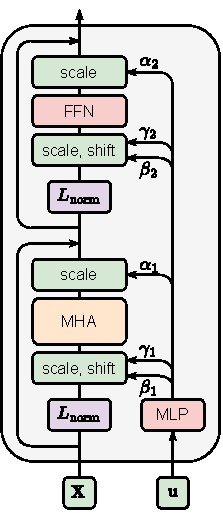
\includegraphics[width=0.25\textwidth]{Figures/graph_networks/adaptivegating.pdf}
    \caption{A TE block with adaptive normalization and gating to incorporate global information.}
    \label{fig:adaptive_gating}
\end{figure}
